\documentclass[1p]{elsarticle_modified}
%\bibliographystyle{elsarticle-num}

%\usepackage[colorlinks]{hyperref}
%\usepackage{abbrmath_seonhwa} %\Abb, \Ascr, \Acal ,\Abf, \Afrak
\usepackage{amsfonts}
\usepackage{amssymb}
\usepackage{amsmath}
\usepackage{amsthm}
\usepackage{scalefnt}
\usepackage{amsbsy}
\usepackage{kotex}
\usepackage{caption}
\usepackage{subfig}
\usepackage{color}
\usepackage{graphicx}
\usepackage{xcolor} %% white, black, red, green, blue, cyan, magenta, yellow
\usepackage{float}
\usepackage{setspace}
\usepackage{hyperref}

\usepackage{tikz}
\usetikzlibrary{arrows}

\usepackage{multirow}
\usepackage{array} % fixed length table
\usepackage{hhline}

%%%%%%%%%%%%%%%%%%%%%
\makeatletter
\renewcommand*\env@matrix[1][\arraystretch]{%
	\edef\arraystretch{#1}%
	\hskip -\arraycolsep
	\let\@ifnextchar\new@ifnextchar
	\array{*\c@MaxMatrixCols c}}
\makeatother %https://tex.stackexchange.com/questions/14071/how-can-i-increase-the-line-spacing-in-a-matrix
%%%%%%%%%%%%%%%

\usepackage[normalem]{ulem}

\newcommand{\msout}[1]{\ifmmode\text{\sout{\ensuremath{#1}}}\else\sout{#1}\fi}
%SOURCE: \msout is \stkout macro in https://tex.stackexchange.com/questions/20609/strikeout-in-math-mode

\newcommand{\cancel}[1]{
	\ifmmode
	{\color{red}\msout{#1}}
	\else
	{\color{red}\sout{#1}}
	\fi
}

\newcommand{\add}[1]{
	{\color{blue}\uwave{#1}}
}

\newcommand{\replace}[2]{
	\ifmmode
	{\color{red}\msout{#1}}{\color{blue}\uwave{#2}}
	\else
	{\color{red}\sout{#1}}{\color{blue}\uwave{#2}}
	\fi
}

\newcommand{\Sol}{\mathcal{S}} %segment
\newcommand{\D}{D} %diagram
\newcommand{\A}{\mathcal{A}} %arc


%%%%%%%%%%%%%%%%%%%%%%%%%%%%%5 test

\def\sl{\operatorname{\textup{SL}}(2,\Cbb)}
\def\psl{\operatorname{\textup{PSL}}(2,\Cbb)}
\def\quan{\mkern 1mu \triangleright \mkern 1mu}

\theoremstyle{definition}
\newtheorem{thm}{Theorem}[section]
\newtheorem{prop}[thm]{Proposition}
\newtheorem{lem}[thm]{Lemma}
\newtheorem{ques}[thm]{Question}
\newtheorem{cor}[thm]{Corollary}
\newtheorem{defn}[thm]{Definition}
\newtheorem{exam}[thm]{Example}
\newtheorem{rmk}[thm]{Remark}
\newtheorem{alg}[thm]{Algorithm}

\newcommand{\I}{\sqrt{-1}}
\begin{document}

%\begin{frontmatter}
%
%\title{Boundary parabolic representations of knots up to 8 crossings}
%
%%% Group authors per affiliation:
%\author{Yunhi Cho} 
%\address{Department of Mathematics, University of Seoul, Seoul, Korea}
%\ead{yhcho@uos.ac.kr}
%
%
%\author{Seonhwa Kim} %\fnref{s_kim}}
%\address{Center for Geometry and Physics, Institute for Basic Science, Pohang, 37673, Korea}
%\ead{ryeona17@ibs.re.kr}
%
%\author{Hyuk Kim}
%\address{Department of Mathematical Sciences, Seoul National University, Seoul 08826, Korea}
%\ead{hyukkim@snu.ac.kr}
%
%\author{Seokbeom Yoon}
%\address{Department of Mathematical Sciences, Seoul National University, Seoul, 08826,  Korea}
%\ead{sbyoon15@snu.ac.kr}
%
%\begin{abstract}
%We find all boundary parabolic representation of knots up to 8 crossings.
%
%\end{abstract}
%\begin{keyword}
%    \MSC[2010] 57M25 
%\end{keyword}
%
%\end{frontmatter}

%\linenumbers
%\tableofcontents
%
\newcommand\colored[1]{\textcolor{white}{\rule[-0.35ex]{0.8em}{1.4ex}}\kern-0.8em\color{red} #1}%
%\newcommand\colored[1]{\textcolor{white}{ #1}\kern-2.17ex	\textcolor{white}{ #1}\kern-1.81ex	\textcolor{white}{ #1}\kern-2.15ex\color{red}#1	}

{\Large $\underline{12a_{1082}~(K12a_{1082})}$}

\setlength{\tabcolsep}{10pt}
\renewcommand{\arraystretch}{1.6}
\vspace{1cm}\begin{tabular}{m{100pt}>{\centering\arraybackslash}m{274pt}}
\multirow{5}{120pt}{
	\centering
	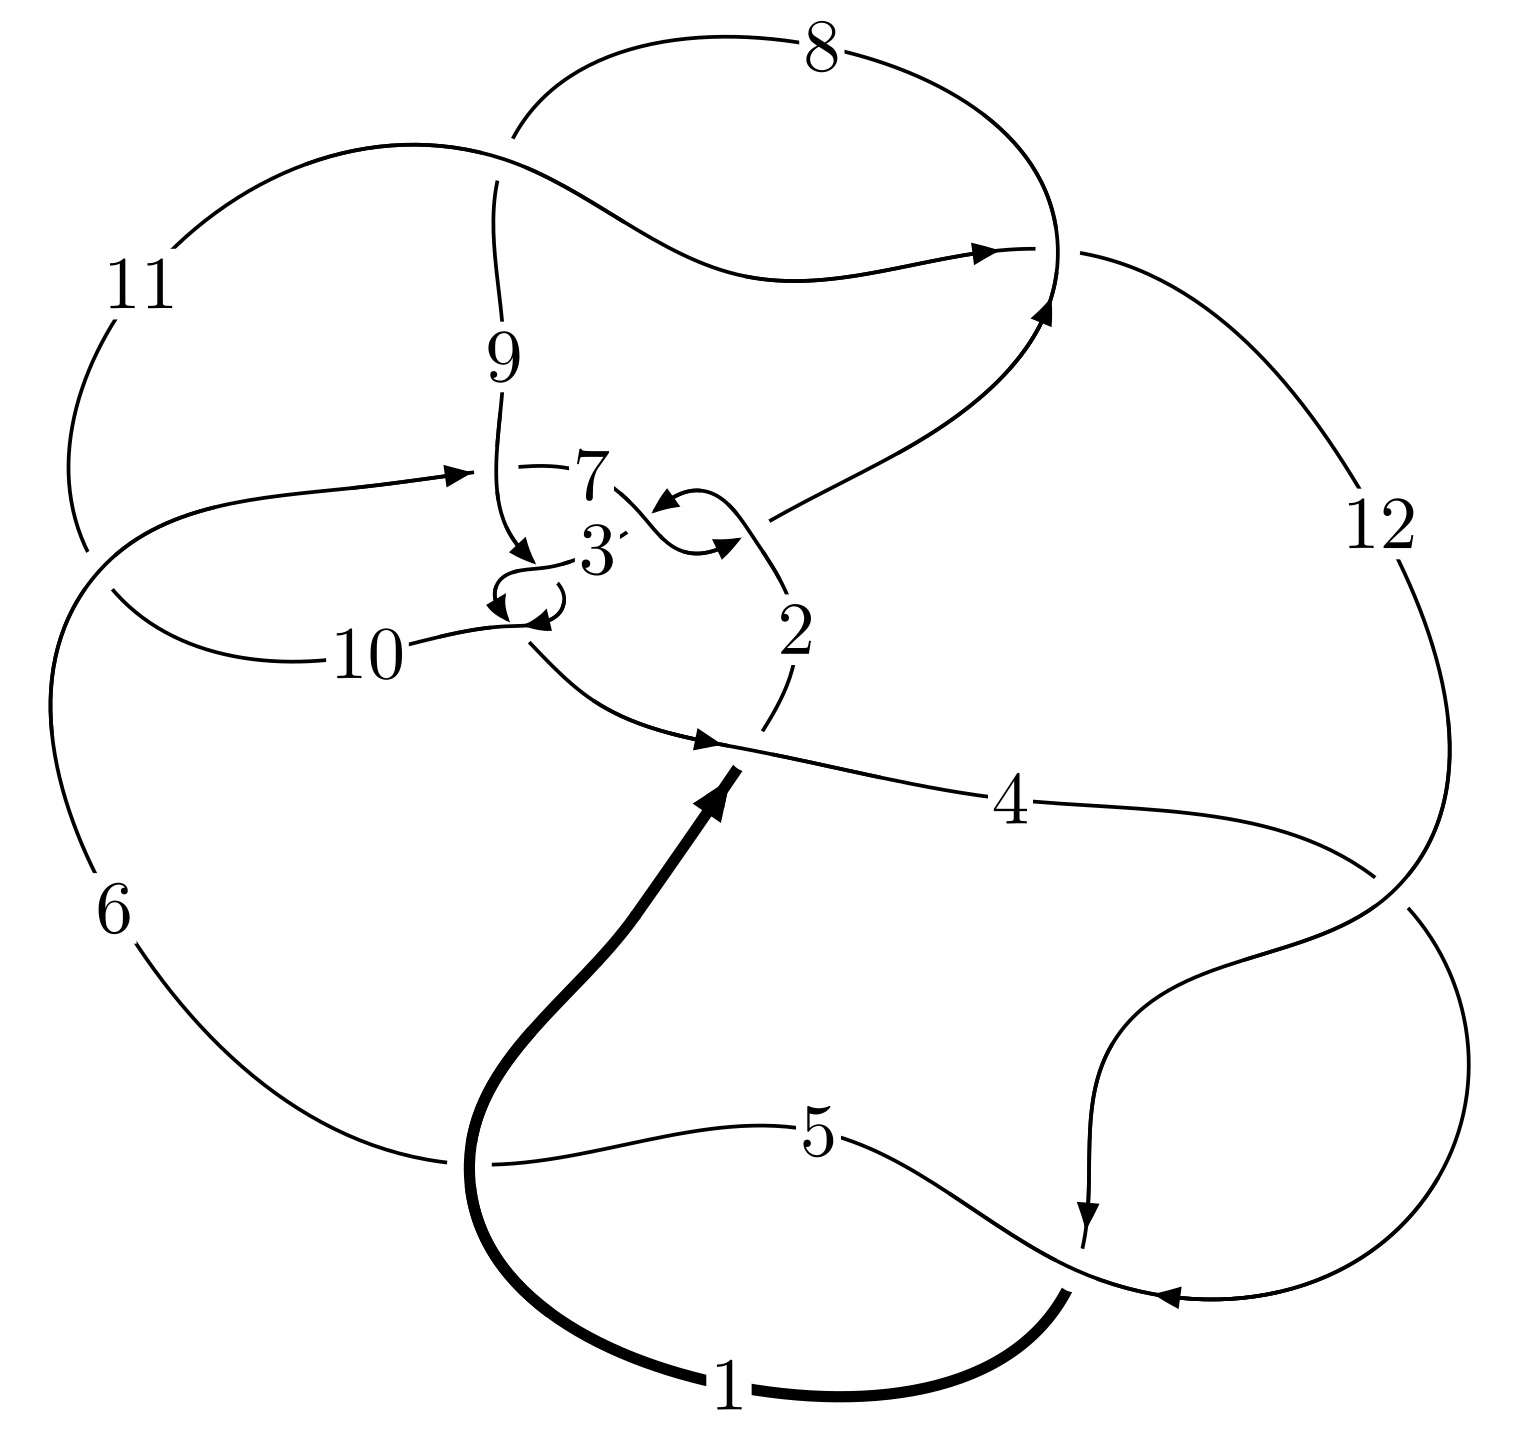
\includegraphics[width=112pt]{../../../GIT/diagram.site/Diagrams/png/1883_12a_1082.png}\\
\ \ \ A knot diagram\footnotemark}&
\allowdisplaybreaks
\textbf{Linearized knot diagam} \\
\cline{2-2}
 &
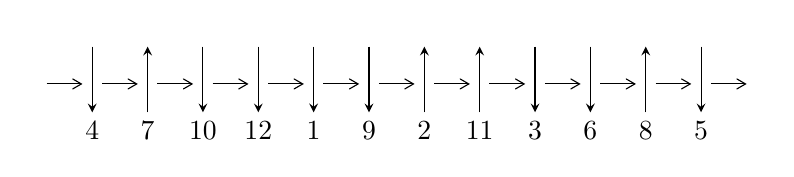
\begin{tikzpicture}[x=20pt, y=17pt]
	% nodes
	\node (C0) at (0, 0) {};
	\node (C1) at (1, 0) {};
	\node (C1U) at (1, +1) {};
	\node (C1D) at (1, -1) {4};

	\node (C2) at (2, 0) {};
	\node (C2U) at (2, +1) {};
	\node (C2D) at (2, -1) {7};

	\node (C3) at (3, 0) {};
	\node (C3U) at (3, +1) {};
	\node (C3D) at (3, -1) {10};

	\node (C4) at (4, 0) {};
	\node (C4U) at (4, +1) {};
	\node (C4D) at (4, -1) {12};

	\node (C5) at (5, 0) {};
	\node (C5U) at (5, +1) {};
	\node (C5D) at (5, -1) {1};

	\node (C6) at (6, 0) {};
	\node (C6U) at (6, +1) {};
	\node (C6D) at (6, -1) {9};

	\node (C7) at (7, 0) {};
	\node (C7U) at (7, +1) {};
	\node (C7D) at (7, -1) {2};

	\node (C8) at (8, 0) {};
	\node (C8U) at (8, +1) {};
	\node (C8D) at (8, -1) {11};

	\node (C9) at (9, 0) {};
	\node (C9U) at (9, +1) {};
	\node (C9D) at (9, -1) {3};

	\node (C10) at (10, 0) {};
	\node (C10U) at (10, +1) {};
	\node (C10D) at (10, -1) {6};

	\node (C11) at (11, 0) {};
	\node (C11U) at (11, +1) {};
	\node (C11D) at (11, -1) {8};

	\node (C12) at (12, 0) {};
	\node (C12U) at (12, +1) {};
	\node (C12D) at (12, -1) {5};
	\node (C13) at (13, 0) {};

	% arrows
	\draw[->,>={angle 60}]
	(C0) edge (C1) (C1) edge (C2) (C2) edge (C3) (C3) edge (C4) (C4) edge (C5) (C5) edge (C6) (C6) edge (C7) (C7) edge (C8) (C8) edge (C9) (C9) edge (C10) (C10) edge (C11) (C11) edge (C12) (C12) edge (C13) ;	\draw[->,>=stealth]
	(C1U) edge (C1D) (C2D) edge (C2U) (C3U) edge (C3D) (C4U) edge (C4D) (C5U) edge (C5D) (C6U) edge (C6D) (C7D) edge (C7U) (C8D) edge (C8U) (C9U) edge (C9D) (C10U) edge (C10D) (C11D) edge (C11U) (C12U) edge (C12D) ;
	\end{tikzpicture} \\
\hhline{~~} \\& 
\textbf{Solving Sequence} \\ \cline{2-2} 
 &
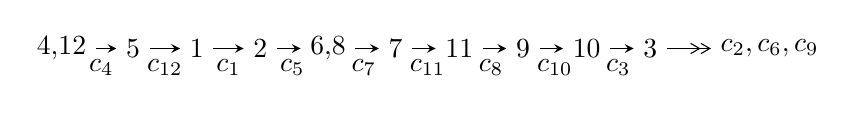
\begin{tikzpicture}[x=23pt, y=7pt]
	% node
	\node (A0) at (-1/8, 0) {4,12};
	\node (A1) at (1, 0) {5};
	\node (A2) at (2, 0) {1};
	\node (A3) at (3, 0) {2};
	\node (A4) at (65/16, 0) {6,8};
	\node (A5) at (41/8, 0) {7};
	\node (A6) at (49/8, 0) {11};
	\node (A7) at (57/8, 0) {9};
	\node (A8) at (65/8, 0) {10};
	\node (A9) at (73/8, 0) {3};
	\node (C1) at (1/2, -1) {$c_{4}$};
	\node (C2) at (3/2, -1) {$c_{12}$};
	\node (C3) at (5/2, -1) {$c_{1}$};
	\node (C4) at (7/2, -1) {$c_{5}$};
	\node (C5) at (37/8, -1) {$c_{7}$};
	\node (C6) at (45/8, -1) {$c_{11}$};
	\node (C7) at (53/8, -1) {$c_{8}$};
	\node (C8) at (61/8, -1) {$c_{10}$};
	\node (C9) at (69/8, -1) {$c_{3}$};
	\node (A10) at (11, 0) {$c_{2},c_{6},c_{9}$};

	% edge
	\draw[->,>=stealth]	
	(A0) edge (A1) (A1) edge (A2) (A2) edge (A3) (A3) edge (A4) (A4) edge (A5) (A5) edge (A6) (A6) edge (A7) (A7) edge (A8) (A8) edge (A9) ;
	\draw[->>,>={angle 60}]	
	(A9) edge (A10);
\end{tikzpicture} \\ 

\end{tabular} \\

\footnotetext{
The image of knot diagram is generated by the software ``\textbf{Draw programme}" developed by Andrew Bartholomew(\url{http://www.layer8.co.uk/maths/draw/index.htm\#Running-draw}), where we modified some parts for our purpose(\url{https://github.com/CATsTAILs/LinksPainter}).
}\phantom \\ \newline 
\centering \textbf{Ideals for irreducible components\footnotemark of $X_{\text{par}}$} 
 
\begin{align*}
I^u_{1}&=\langle 
7.37646\times10^{158} u^{119}+1.70979\times10^{159} u^{118}+\cdots+9.35321\times10^{158} b+5.75418\times10^{158},\\
\phantom{I^u_{1}}&\phantom{= \langle  }1.29225\times10^{159} u^{119}+3.14232\times10^{159} u^{118}+\cdots+9.35321\times10^{158} a-2.96601\times10^{159},\;u^{120}+3 u^{119}+\cdots+8 u-1\rangle \\
I^u_{2}&=\langle 
-2 u^{27}+2 u^{26}+\cdots+b+2,\;-6 u^{27}+6 u^{26}+\cdots+a-8 u,\;u^{28}-2 u^{27}+\cdots-2 u+1\rangle \\
\\
\end{align*}
\raggedright * 2 irreducible components of $\dim_{\mathbb{C}}=0$, with total 148 representations.\\
\footnotetext{All coefficients of polynomials are rational numbers. But the coefficients are sometimes approximated in decimal forms when there is not enough margin.}
\newpage
\renewcommand{\arraystretch}{1}
\centering \section*{I. $I^u_{1}= \langle 7.38\times10^{158} u^{119}+1.71\times10^{159} u^{118}+\cdots+9.35\times10^{158} b+5.75\times10^{158},\;1.29\times10^{159} u^{119}+3.14\times10^{159} u^{118}+\cdots+9.35\times10^{158} a-2.97\times10^{159},\;u^{120}+3 u^{119}+\cdots+8 u-1 \rangle$}
\flushleft \textbf{(i) Arc colorings}\\
\begin{tabular}{m{7pt} m{180pt} m{7pt} m{180pt} }
\flushright $a_{4}=$&$\begin{pmatrix}1\\0\end{pmatrix}$ \\
\flushright $a_{12}=$&$\begin{pmatrix}0\\u\end{pmatrix}$ \\
\flushright $a_{5}=$&$\begin{pmatrix}1\\u^2\end{pmatrix}$ \\
\flushright $a_{1}=$&$\begin{pmatrix}- u\\- u^3+u\end{pmatrix}$ \\
\flushright $a_{2}=$&$\begin{pmatrix}u^3-2 u\\- u^3+u\end{pmatrix}$ \\
\flushright $a_{6}=$&$\begin{pmatrix}- u^2+1\\- u^4+2 u^2\end{pmatrix}$ \\
\flushright $a_{8}=$&$\begin{pmatrix}-1.38161 u^{119}-3.35961 u^{118}+\cdots+51.8433 u+3.17111\\-0.788655 u^{119}-1.82803 u^{118}+\cdots+23.3617 u-0.615209\end{pmatrix}$ \\
\flushright $a_{7}=$&$\begin{pmatrix}-2.07596 u^{119}-4.65251 u^{118}+\cdots+49.1162 u+3.92968\\-2.17737 u^{119}-4.16193 u^{118}+\cdots+13.1942 u+0.316698\end{pmatrix}$ \\
\flushright $a_{11}=$&$\begin{pmatrix}-0.0726298 u^{119}-0.187189 u^{118}+\cdots-39.6037 u+6.85858\\2.27088 u^{119}+3.37252 u^{118}+\cdots+13.7032 u+0.133101\end{pmatrix}$ \\
\flushright $a_{9}=$&$\begin{pmatrix}2.01690 u^{119}+3.70837 u^{118}+\cdots+3.84406 u+4.68181\\-0.381437 u^{119}-0.853970 u^{118}+\cdots+10.7822 u+0.480982\end{pmatrix}$ \\
\flushright $a_{10}=$&$\begin{pmatrix}1.73603 u^{119}+3.47491 u^{118}+\cdots-35.1363 u+8.10741\\-0.0452228 u^{119}-0.441756 u^{118}+\cdots+3.24667 u+1.38489\end{pmatrix}$ \\
\flushright $a_{3}=$&$\begin{pmatrix}2.44612 u^{119}+3.70156 u^{118}+\cdots+72.8518 u-14.1062\\0.640744 u^{119}+2.05119 u^{118}+\cdots-4.49843 u-1.93172\end{pmatrix}$\\&\end{tabular}
\flushleft \textbf{(ii) Obstruction class $= -1$}\\~\\
\flushleft \textbf{(iii) Cusp Shapes $= 2.90682 u^{119}+8.84972 u^{118}+\cdots-6.43341 u-13.9528$}\\~\\
\newpage\renewcommand{\arraystretch}{1}
\flushleft \textbf{(iv) u-Polynomials at the component}\newline \\
\begin{tabular}{m{50pt}|m{274pt}}
Crossings & \hspace{64pt}u-Polynomials at each crossing \\
\hline $$\begin{aligned}c_{1}\end{aligned}$$&$\begin{aligned}
&u^{120}-9 u^{119}+\cdots-3718 u+2197
\end{aligned}$\\
\hline $$\begin{aligned}c_{2},c_{7}\end{aligned}$$&$\begin{aligned}
&u^{120}+u^{119}+\cdots+505942 u-143161
\end{aligned}$\\
\hline $$\begin{aligned}c_{3},c_{9}\end{aligned}$$&$\begin{aligned}
&u^{120}+u^{119}+\cdots-497 u-991
\end{aligned}$\\
\hline $$\begin{aligned}c_{4},c_{5},c_{12}\end{aligned}$$&$\begin{aligned}
&u^{120}+3 u^{119}+\cdots+8 u-1
\end{aligned}$\\
\hline $$\begin{aligned}c_{6}\end{aligned}$$&$\begin{aligned}
&u^{120}-6 u^{119}+\cdots-111403235 u+12357323
\end{aligned}$\\
\hline $$\begin{aligned}c_{8},c_{11}\end{aligned}$$&$\begin{aligned}
&u^{120}+6 u^{119}+\cdots+64698 u+4996
\end{aligned}$\\
\hline $$\begin{aligned}c_{10}\end{aligned}$$&$\begin{aligned}
&u^{120}+2 u^{119}+\cdots+86310 u+45641
\end{aligned}$\\
\hline
\end{tabular}\\~\\
\newpage\renewcommand{\arraystretch}{1}
\flushleft \textbf{(v) Riley Polynomials at the component}\newline \\
\begin{tabular}{m{50pt}|m{274pt}}
Crossings & \hspace{64pt}Riley Polynomials at each crossing \\
\hline $$\begin{aligned}c_{1}\end{aligned}$$&$\begin{aligned}
&y^{120}-3 y^{119}+\cdots+654218266 y+4826809
\end{aligned}$\\
\hline $$\begin{aligned}c_{2},c_{7}\end{aligned}$$&$\begin{aligned}
&y^{120}+103 y^{119}+\cdots+401123665620 y+20495071921
\end{aligned}$\\
\hline $$\begin{aligned}c_{3},c_{9}\end{aligned}$$&$\begin{aligned}
&y^{120}-85 y^{119}+\cdots-45176967 y+982081
\end{aligned}$\\
\hline $$\begin{aligned}c_{4},c_{5},c_{12}\end{aligned}$$&$\begin{aligned}
&y^{120}-111 y^{119}+\cdots+160 y+1
\end{aligned}$\\
\hline $$\begin{aligned}c_{6}\end{aligned}$$&$\begin{aligned}
&y^{120}-54 y^{119}+\cdots-7346690606945771 y+152703431726329
\end{aligned}$\\
\hline $$\begin{aligned}c_{8},c_{11}\end{aligned}$$&$\begin{aligned}
&y^{120}+82 y^{119}+\cdots+638456276 y+24960016
\end{aligned}$\\
\hline $$\begin{aligned}c_{10}\end{aligned}$$&$\begin{aligned}
&y^{120}-32 y^{119}+\cdots-57169443552 y+2083100881
\end{aligned}$\\
\hline
\end{tabular}\\~\\
\newpage\flushleft \textbf{(vi) Complex Volumes and Cusp Shapes}
$$\begin{array}{c|c|c}  
\text{Solutions to }I^u_{1}& \I (\text{vol} + \sqrt{-1}CS) & \text{Cusp shape}\\
 \hline 
\begin{aligned}
u &= \phantom{-}0.758063 + 0.612639 I \\
a &= -1.22294 - 0.75012 I \\
b &= \phantom{-}0.470196 - 0.508802 I\end{aligned}
 & -9.18918 + 8.98662 I & \phantom{-0.000000 } 0 \\ \hline\begin{aligned}
u &= \phantom{-}0.758063 - 0.612639 I \\
a &= -1.22294 + 0.75012 I \\
b &= \phantom{-}0.470196 + 0.508802 I\end{aligned}
 & -9.18918 - 8.98662 I & \phantom{-0.000000 } 0 \\ \hline\begin{aligned}
u &= -0.995734 + 0.272083 I \\
a &= \phantom{-}0.138623 + 1.054390 I \\
b &= \phantom{-}0.907901 - 0.711733 I\end{aligned}
 & -4.04811 + 3.42712 I & \phantom{-0.000000 } 0 \\ \hline\begin{aligned}
u &= -0.995734 - 0.272083 I \\
a &= \phantom{-}0.138623 - 1.054390 I \\
b &= \phantom{-}0.907901 + 0.711733 I\end{aligned}
 & -4.04811 - 3.42712 I & \phantom{-0.000000 } 0 \\ \hline\begin{aligned}
u &= \phantom{-}0.614537 + 0.723379 I \\
a &= -0.382409 - 0.933491 I \\
b &= \phantom{-}0.520893 + 0.967316 I\end{aligned}
 & -2.87584 - 4.39613 I & \phantom{-0.000000 } 0 \\ \hline\begin{aligned}
u &= \phantom{-}0.614537 - 0.723379 I \\
a &= -0.382409 + 0.933491 I \\
b &= \phantom{-}0.520893 - 0.967316 I\end{aligned}
 & -2.87584 + 4.39613 I & \phantom{-0.000000 } 0 \\ \hline\begin{aligned}
u &= -0.160696 + 0.922940 I \\
a &= -1.051960 + 0.231090 I \\
b &= \phantom{-}1.049000 - 0.295188 I\end{aligned}
 & -1.37343 + 2.15773 I & \phantom{-0.000000 } 0 \\ \hline\begin{aligned}
u &= -0.160696 - 0.922940 I \\
a &= -1.051960 - 0.231090 I \\
b &= \phantom{-}1.049000 + 0.295188 I\end{aligned}
 & -1.37343 - 2.15773 I & \phantom{-0.000000 } 0 \\ \hline\begin{aligned}
u &= -1.058680 + 0.145296 I \\
a &= \phantom{-}0.460538 + 0.227295 I \\
b &= \phantom{-}0.840560 - 0.207999 I\end{aligned}
 & -1.56282 + 0.11358 I & \phantom{-0.000000 } 0 \\ \hline\begin{aligned}
u &= -1.058680 - 0.145296 I \\
a &= \phantom{-}0.460538 - 0.227295 I \\
b &= \phantom{-}0.840560 + 0.207999 I\end{aligned}
 & -1.56282 - 0.11358 I & \phantom{-0.000000 } 0\\
 \hline 
 \end{array}$$\newpage$$\begin{array}{c|c|c}  
\text{Solutions to }I^u_{1}& \I (\text{vol} + \sqrt{-1}CS) & \text{Cusp shape}\\
 \hline 
\begin{aligned}
u &= -0.771663 + 0.446424 I \\
a &= -1.14604 + 1.04772 I \\
b &= \phantom{-}0.541922 + 0.544394 I\end{aligned}
 & -4.96355 - 3.50876 I & \phantom{-0.000000 } 0 \\ \hline\begin{aligned}
u &= -0.771663 - 0.446424 I \\
a &= -1.14604 - 1.04772 I \\
b &= \phantom{-}0.541922 - 0.544394 I\end{aligned}
 & -4.96355 + 3.50876 I & \phantom{-0.000000 } 0 \\ \hline\begin{aligned}
u &= \phantom{-}0.357261 + 0.813565 I \\
a &= \phantom{-}1.15745 + 1.19649 I \\
b &= -1.19712 - 1.22505 I\end{aligned}
 & -7.9239 - 13.8663 I & \phantom{-0.000000 } 0 \\ \hline\begin{aligned}
u &= \phantom{-}0.357261 - 0.813565 I \\
a &= \phantom{-}1.15745 - 1.19649 I \\
b &= -1.19712 + 1.22505 I\end{aligned}
 & -7.9239 + 13.8663 I & \phantom{-0.000000 } 0 \\ \hline\begin{aligned}
u &= -0.404133 + 0.783971 I \\
a &= -0.866155 + 0.697337 I \\
b &= \phantom{-}0.748223 - 0.769256 I\end{aligned}
 & -1.51097 + 2.78695 I & \phantom{-0.000000 } 0 \\ \hline\begin{aligned}
u &= -0.404133 - 0.783971 I \\
a &= -0.866155 - 0.697337 I \\
b &= \phantom{-}0.748223 + 0.769256 I\end{aligned}
 & -1.51097 - 2.78695 I & \phantom{-0.000000 } 0 \\ \hline\begin{aligned}
u &= \phantom{-}1.094700 + 0.234164 I \\
a &= -0.577419 - 0.264483 I \\
b &= -0.549890 + 0.527872 I\end{aligned}
 & -4.54668 - 4.46609 I & \phantom{-0.000000 } 0 \\ \hline\begin{aligned}
u &= \phantom{-}1.094700 - 0.234164 I \\
a &= -0.577419 + 0.264483 I \\
b &= -0.549890 - 0.527872 I\end{aligned}
 & -4.54668 + 4.46609 I & \phantom{-0.000000 } 0 \\ \hline\begin{aligned}
u &= -1.033800 + 0.437885 I \\
a &= \phantom{-}0.257491 - 0.940473 I \\
b &= -0.686255 - 0.343745 I\end{aligned}
 & -4.07515 + 2.66051 I & \phantom{-0.000000 } 0 \\ \hline\begin{aligned}
u &= -1.033800 - 0.437885 I \\
a &= \phantom{-}0.257491 + 0.940473 I \\
b &= -0.686255 + 0.343745 I\end{aligned}
 & -4.07515 - 2.66051 I & \phantom{-0.000000 } 0\\
 \hline 
 \end{array}$$\newpage$$\begin{array}{c|c|c}  
\text{Solutions to }I^u_{1}& \I (\text{vol} + \sqrt{-1}CS) & \text{Cusp shape}\\
 \hline 
\begin{aligned}
u &= \phantom{-}1.131310 + 0.055315 I \\
a &= -0.151277 + 0.933019 I \\
b &= \phantom{-}0.13358 + 1.85091 I\end{aligned}
 & -9.53618 + 0.93120 I & \phantom{-0.000000 } 0 \\ \hline\begin{aligned}
u &= \phantom{-}1.131310 - 0.055315 I \\
a &= -0.151277 - 0.933019 I \\
b &= \phantom{-}0.13358 - 1.85091 I\end{aligned}
 & -9.53618 - 0.93120 I & \phantom{-0.000000 } 0 \\ \hline\begin{aligned}
u &= -0.440237 + 0.713965 I \\
a &= \phantom{-}0.992326 - 0.668774 I \\
b &= -0.325618 + 0.204381 I\end{aligned}
 & -1.69555 + 1.98381 I & \phantom{-0.000000 } 0 \\ \hline\begin{aligned}
u &= -0.440237 - 0.713965 I \\
a &= \phantom{-}0.992326 + 0.668774 I \\
b &= -0.325618 - 0.204381 I\end{aligned}
 & -1.69555 - 1.98381 I & \phantom{-0.000000 } 0 \\ \hline\begin{aligned}
u &= \phantom{-}0.347045 + 0.743011 I \\
a &= \phantom{-}0.869436 - 0.335291 I \\
b &= -0.018759 + 0.573045 I\end{aligned}
 & -2.03680 - 0.36310 I & \phantom{-0.000000 } 0 \\ \hline\begin{aligned}
u &= \phantom{-}0.347045 - 0.743011 I \\
a &= \phantom{-}0.869436 + 0.335291 I \\
b &= -0.018759 - 0.573045 I\end{aligned}
 & -2.03680 + 0.36310 I & \phantom{-0.000000 } 0 \\ \hline\begin{aligned}
u &= -0.296638 + 0.762588 I \\
a &= \phantom{-}1.32323 - 1.27789 I \\
b &= -1.33073 + 1.15712 I\end{aligned}
 & -3.39639 + 7.81505 I & \phantom{-0.000000 } 0 \\ \hline\begin{aligned}
u &= -0.296638 - 0.762588 I \\
a &= \phantom{-}1.32323 + 1.27789 I \\
b &= -1.33073 - 1.15712 I\end{aligned}
 & -3.39639 - 7.81505 I & \phantom{-0.000000 } 0 \\ \hline\begin{aligned}
u &= \phantom{-}1.193810 + 0.072843 I \\
a &= \phantom{-}0.616469 + 0.767214 I \\
b &= \phantom{-}0.758914 + 0.153228 I\end{aligned}
 & -2.23354 + 1.52529 I & \phantom{-0.000000 } 0 \\ \hline\begin{aligned}
u &= \phantom{-}1.193810 - 0.072843 I \\
a &= \phantom{-}0.616469 - 0.767214 I \\
b &= \phantom{-}0.758914 - 0.153228 I\end{aligned}
 & -2.23354 - 1.52529 I & \phantom{-0.000000 } 0\\
 \hline 
 \end{array}$$\newpage$$\begin{array}{c|c|c}  
\text{Solutions to }I^u_{1}& \I (\text{vol} + \sqrt{-1}CS) & \text{Cusp shape}\\
 \hline 
\begin{aligned}
u &= -0.045115 + 0.792707 I \\
a &= \phantom{-}0.995941 + 0.391751 I \\
b &= -0.248171 - 0.528968 I\end{aligned}
 & -1.174710 + 0.610806 I & -5.85025 + 1.21411 I \\ \hline\begin{aligned}
u &= -0.045115 - 0.792707 I \\
a &= \phantom{-}0.995941 - 0.391751 I \\
b &= -0.248171 + 0.528968 I\end{aligned}
 & -1.174710 - 0.610806 I & -5.85025 - 1.21411 I \\ \hline\begin{aligned}
u &= -1.213260 + 0.074521 I \\
a &= -0.738681 - 0.552826 I \\
b &= -0.95568 + 1.47398 I\end{aligned}
 & -2.10913 + 0.80254 I & \phantom{-0.000000 } 0 \\ \hline\begin{aligned}
u &= -1.213260 - 0.074521 I \\
a &= -0.738681 + 0.552826 I \\
b &= -0.95568 - 1.47398 I\end{aligned}
 & -2.10913 - 0.80254 I & \phantom{-0.000000 } 0 \\ \hline\begin{aligned}
u &= -0.714265 + 0.257828 I \\
a &= \phantom{-}0.95188 - 1.20880 I \\
b &= \phantom{-}0.284028 + 0.353544 I\end{aligned}
 & -4.34819 - 3.50064 I & -10.15879 + 2.61062 I \\ \hline\begin{aligned}
u &= -0.714265 - 0.257828 I \\
a &= \phantom{-}0.95188 + 1.20880 I \\
b &= \phantom{-}0.284028 - 0.353544 I\end{aligned}
 & -4.34819 + 3.50064 I & -10.15879 - 2.61062 I \\ \hline\begin{aligned}
u &= -0.267217 + 0.705736 I \\
a &= -1.37518 + 1.03742 I \\
b &= \phantom{-}0.584151 - 1.234020 I\end{aligned}
 & -2.73124 + 7.20564 I & -7.22129 - 8.23166 I \\ \hline\begin{aligned}
u &= -0.267217 - 0.705736 I \\
a &= -1.37518 - 1.03742 I \\
b &= \phantom{-}0.584151 + 1.234020 I\end{aligned}
 & -2.73124 - 7.20564 I & -7.22129 + 8.23166 I \\ \hline\begin{aligned}
u &= \phantom{-}0.293364 + 0.692080 I \\
a &= -0.65992 + 1.40520 I \\
b &= -0.22122 - 1.46251 I\end{aligned}
 & -3.72611 - 7.81436 I & -5.94311 + 7.27559 I \\ \hline\begin{aligned}
u &= \phantom{-}0.293364 - 0.692080 I \\
a &= -0.65992 - 1.40520 I \\
b &= -0.22122 + 1.46251 I\end{aligned}
 & -3.72611 + 7.81436 I & -5.94311 - 7.27559 I\\
 \hline 
 \end{array}$$\newpage$$\begin{array}{c|c|c}  
\text{Solutions to }I^u_{1}& \I (\text{vol} + \sqrt{-1}CS) & \text{Cusp shape}\\
 \hline 
\begin{aligned}
u &= -0.164096 + 0.720950 I \\
a &= \phantom{-}0.242278 + 0.831725 I \\
b &= -0.196291 - 0.953290 I\end{aligned}
 & \phantom{-}0.96231 + 3.37259 I & -0.66181 - 5.02684 I \\ \hline\begin{aligned}
u &= -0.164096 - 0.720950 I \\
a &= \phantom{-}0.242278 - 0.831725 I \\
b &= -0.196291 + 0.953290 I\end{aligned}
 & \phantom{-}0.96231 - 3.37259 I & -0.66181 + 5.02684 I \\ \hline\begin{aligned}
u &= \phantom{-}1.255140 + 0.207604 I \\
a &= \phantom{-}0.600745 - 0.538593 I \\
b &= \phantom{-}1.30795 + 0.56083 I\end{aligned}
 & -0.95909 - 4.01812 I & \phantom{-0.000000 } 0 \\ \hline\begin{aligned}
u &= \phantom{-}1.255140 - 0.207604 I \\
a &= \phantom{-}0.600745 + 0.538593 I \\
b &= \phantom{-}1.30795 - 0.56083 I\end{aligned}
 & -0.95909 + 4.01812 I & \phantom{-0.000000 } 0 \\ \hline\begin{aligned}
u &= -0.719676\phantom{ +0.000000I} \\
a &= \phantom{-}0.701794\phantom{ +0.000000I} \\
b &= \phantom{-}0.424952\phantom{ +0.000000I}\end{aligned}
 & -1.50335\phantom{ +0.000000I} & -6.04810\phantom{ +0.000000I} \\ \hline\begin{aligned}
u &= -1.273630 + 0.227101 I \\
a &= -0.623129 + 0.007221 I \\
b &= -0.024009 + 1.071650 I\end{aligned}
 & -1.12960 + 2.12830 I & \phantom{-0.000000 } 0 \\ \hline\begin{aligned}
u &= -1.273630 - 0.227101 I \\
a &= -0.623129 - 0.007221 I \\
b &= -0.024009 - 1.071650 I\end{aligned}
 & -1.12960 - 2.12830 I & \phantom{-0.000000 } 0 \\ \hline\begin{aligned}
u &= \phantom{-}0.297171 + 0.631786 I \\
a &= \phantom{-}1.29874 + 1.61569 I \\
b &= -1.50993 - 1.26578 I\end{aligned}
 & -8.12476 - 1.41435 I & -10.19810 + 3.32175 I \\ \hline\begin{aligned}
u &= \phantom{-}0.297171 - 0.631786 I \\
a &= \phantom{-}1.29874 - 1.61569 I \\
b &= -1.50993 + 1.26578 I\end{aligned}
 & -8.12476 + 1.41435 I & -10.19810 - 3.32175 I \\ \hline\begin{aligned}
u &= \phantom{-}0.593856 + 0.322694 I \\
a &= -1.144100 + 0.499841 I \\
b &= -0.117888 - 1.239260 I\end{aligned}
 & -5.01452 + 4.11784 I & -8.48824 - 1.68058 I\\
 \hline 
 \end{array}$$\newpage$$\begin{array}{c|c|c}  
\text{Solutions to }I^u_{1}& \I (\text{vol} + \sqrt{-1}CS) & \text{Cusp shape}\\
 \hline 
\begin{aligned}
u &= \phantom{-}0.593856 - 0.322694 I \\
a &= -1.144100 - 0.499841 I \\
b &= -0.117888 + 1.239260 I\end{aligned}
 & -5.01452 - 4.11784 I & -8.48824 + 1.68058 I \\ \hline\begin{aligned}
u &= \phantom{-}0.235947 + 0.623765 I \\
a &= -1.57054 - 0.72572 I \\
b &= \phantom{-}1.60485 + 1.23476 I\end{aligned}
 & -7.32776 - 3.51777 I & -11.20872 + 5.37878 I \\ \hline\begin{aligned}
u &= \phantom{-}0.235947 - 0.623765 I \\
a &= -1.57054 + 0.72572 I \\
b &= \phantom{-}1.60485 - 1.23476 I\end{aligned}
 & -7.32776 + 3.51777 I & -11.20872 - 5.37878 I \\ \hline\begin{aligned}
u &= \phantom{-}1.338000 + 0.055970 I \\
a &= -0.097785 - 1.142750 I \\
b &= -0.57344 + 1.56737 I\end{aligned}
 & -11.78960 - 1.92476 I & \phantom{-0.000000 } 0 \\ \hline\begin{aligned}
u &= \phantom{-}1.338000 - 0.055970 I \\
a &= -0.097785 + 1.142750 I \\
b &= -0.57344 - 1.56737 I\end{aligned}
 & -11.78960 + 1.92476 I & \phantom{-0.000000 } 0 \\ \hline\begin{aligned}
u &= \phantom{-}0.012576 + 0.632373 I \\
a &= \phantom{-}0.577328 - 1.252450 I \\
b &= -0.562925 + 0.991272 I\end{aligned}
 & \phantom{-}2.83723 + 0.97754 I & \phantom{-}3.54382 - 2.20940 I \\ \hline\begin{aligned}
u &= \phantom{-}0.012576 - 0.632373 I \\
a &= \phantom{-}0.577328 + 1.252450 I \\
b &= -0.562925 - 0.991272 I\end{aligned}
 & \phantom{-}2.83723 - 0.97754 I & \phantom{-}3.54382 + 2.20940 I \\ \hline\begin{aligned}
u &= \phantom{-}1.352470 + 0.213334 I \\
a &= -0.414971 - 0.200004 I \\
b &= -0.860846 - 0.278696 I\end{aligned}
 & -5.08107 - 3.53397 I & \phantom{-0.000000 } 0 \\ \hline\begin{aligned}
u &= \phantom{-}1.352470 - 0.213334 I \\
a &= -0.414971 + 0.200004 I \\
b &= -0.860846 + 0.278696 I\end{aligned}
 & -5.08107 + 3.53397 I & \phantom{-0.000000 } 0 \\ \hline\begin{aligned}
u &= \phantom{-}0.230584 + 0.580687 I \\
a &= -1.42586 - 1.37552 I \\
b &= \phantom{-}0.552732 + 1.125940 I\end{aligned}
 & \phantom{-}0.27877 - 3.72484 I & -0.25287 + 3.53714 I\\
 \hline 
 \end{array}$$\newpage$$\begin{array}{c|c|c}  
\text{Solutions to }I^u_{1}& \I (\text{vol} + \sqrt{-1}CS) & \text{Cusp shape}\\
 \hline 
\begin{aligned}
u &= \phantom{-}0.230584 - 0.580687 I \\
a &= -1.42586 + 1.37552 I \\
b &= \phantom{-}0.552732 - 1.125940 I\end{aligned}
 & \phantom{-}0.27877 + 3.72484 I & -0.25287 - 3.53714 I \\ \hline\begin{aligned}
u &= \phantom{-}1.351520 + 0.300209 I \\
a &= -0.439642 + 0.118954 I \\
b &= -0.352361 - 1.056070 I\end{aligned}
 & -3.81291 - 7.07815 I & \phantom{-0.000000 } 0 \\ \hline\begin{aligned}
u &= \phantom{-}1.351520 - 0.300209 I \\
a &= -0.439642 - 0.118954 I \\
b &= -0.352361 + 1.056070 I\end{aligned}
 & -3.81291 + 7.07815 I & \phantom{-0.000000 } 0 \\ \hline\begin{aligned}
u &= -1.377860 + 0.198340 I \\
a &= -0.092721 + 0.816913 I \\
b &= \phantom{-}1.33537 - 1.57047 I\end{aligned}
 & -5.39823 + 1.12081 I & \phantom{-0.000000 } 0 \\ \hline\begin{aligned}
u &= -1.377860 - 0.198340 I \\
a &= -0.092721 - 0.816913 I \\
b &= \phantom{-}1.33537 + 1.57047 I\end{aligned}
 & -5.39823 - 1.12081 I & \phantom{-0.000000 } 0 \\ \hline\begin{aligned}
u &= \phantom{-}1.39625\phantom{ +0.000000I} \\
a &= -0.427157\phantom{ +0.000000I} \\
b &= \phantom{-}0.0766782\phantom{ +0.000000I}\end{aligned}
 & -7.75893\phantom{ +0.000000I} & \phantom{-0.000000 } 0 \\ \hline\begin{aligned}
u &= \phantom{-}1.308430 + 0.495916 I \\
a &= \phantom{-}0.136018 + 0.735283 I \\
b &= -1.094890 - 0.176787 I\end{aligned}
 & -5.94181 - 7.24846 I & \phantom{-0.000000 } 0 \\ \hline\begin{aligned}
u &= \phantom{-}1.308430 - 0.495916 I \\
a &= \phantom{-}0.136018 - 0.735283 I \\
b &= -1.094890 + 0.176787 I\end{aligned}
 & -5.94181 + 7.24846 I & \phantom{-0.000000 } 0 \\ \hline\begin{aligned}
u &= -1.397780 + 0.124154 I \\
a &= -0.214087 + 0.312942 I \\
b &= -1.87470 + 0.94938 I\end{aligned}
 & -10.21350 + 4.66937 I & \phantom{-0.000000 } 0 \\ \hline\begin{aligned}
u &= -1.397780 - 0.124154 I \\
a &= -0.214087 - 0.312942 I \\
b &= -1.87470 - 0.94938 I\end{aligned}
 & -10.21350 - 4.66937 I & \phantom{-0.000000 } 0\\
 \hline 
 \end{array}$$\newpage$$\begin{array}{c|c|c}  
\text{Solutions to }I^u_{1}& \I (\text{vol} + \sqrt{-1}CS) & \text{Cusp shape}\\
 \hline 
\begin{aligned}
u &= \phantom{-}1.399710 + 0.129687 I \\
a &= -0.122996 - 0.787009 I \\
b &= \phantom{-}1.25500 + 2.69944 I\end{aligned}
 & -10.24600 + 2.33584 I & \phantom{-0.000000 } 0 \\ \hline\begin{aligned}
u &= \phantom{-}1.399710 - 0.129687 I \\
a &= -0.122996 + 0.787009 I \\
b &= \phantom{-}1.25500 - 2.69944 I\end{aligned}
 & -10.24600 - 2.33584 I & \phantom{-0.000000 } 0 \\ \hline\begin{aligned}
u &= -1.394160 + 0.180221 I \\
a &= -0.223833 + 1.000450 I \\
b &= -0.36504 - 1.80456 I\end{aligned}
 & -13.52120 + 1.36381 I & \phantom{-0.000000 } 0 \\ \hline\begin{aligned}
u &= -1.394160 - 0.180221 I \\
a &= -0.223833 - 1.000450 I \\
b &= -0.36504 + 1.80456 I\end{aligned}
 & -13.52120 - 1.36381 I & \phantom{-0.000000 } 0 \\ \hline\begin{aligned}
u &= -1.390760 + 0.230878 I \\
a &= -0.152323 - 0.959451 I \\
b &= -1.59968 + 1.94546 I\end{aligned}
 & -4.90359 + 6.72120 I & \phantom{-0.000000 } 0 \\ \hline\begin{aligned}
u &= -1.390760 - 0.230878 I \\
a &= -0.152323 + 0.959451 I \\
b &= -1.59968 - 1.94546 I\end{aligned}
 & -4.90359 - 6.72120 I & \phantom{-0.000000 } 0 \\ \hline\begin{aligned}
u &= \phantom{-}1.393660 + 0.218126 I \\
a &= \phantom{-}1.111440 + 0.019269 I \\
b &= \phantom{-}0.60142 + 1.46469 I\end{aligned}
 & -4.60265 - 4.02663 I & \phantom{-0.000000 } 0 \\ \hline\begin{aligned}
u &= \phantom{-}1.393660 - 0.218126 I \\
a &= \phantom{-}1.111440 - 0.019269 I \\
b &= \phantom{-}0.60142 - 1.46469 I\end{aligned}
 & -4.60265 + 4.02663 I & \phantom{-0.000000 } 0 \\ \hline\begin{aligned}
u &= -0.229473 + 0.539634 I \\
a &= -1.28148 - 1.86660 I \\
b &= -0.06183 + 1.62357 I\end{aligned}
 & \phantom{-}0.606565 + 1.201870 I & -10.56206 - 6.88957 I \\ \hline\begin{aligned}
u &= -0.229473 - 0.539634 I \\
a &= -1.28148 + 1.86660 I \\
b &= -0.06183 - 1.62357 I\end{aligned}
 & \phantom{-}0.606565 - 1.201870 I & -10.56206 + 6.88957 I\\
 \hline 
 \end{array}$$\newpage$$\begin{array}{c|c|c}  
\text{Solutions to }I^u_{1}& \I (\text{vol} + \sqrt{-1}CS) & \text{Cusp shape}\\
 \hline 
\begin{aligned}
u &= -1.39466 + 0.24727 I \\
a &= \phantom{-}0.001851 - 0.833863 I \\
b &= -3.08790 + 0.93606 I\end{aligned}
 & -12.5379 + 6.7134 I & \phantom{-0.000000 } 0 \\ \hline\begin{aligned}
u &= -1.39466 - 0.24727 I \\
a &= \phantom{-}0.001851 + 0.833863 I \\
b &= -3.08790 - 0.93606 I\end{aligned}
 & -12.5379 - 6.7134 I & \phantom{-0.000000 } 0 \\ \hline\begin{aligned}
u &= \phantom{-}1.42192 + 0.10390 I \\
a &= -0.303312 + 0.815867 I \\
b &= -1.49389 - 1.92620 I\end{aligned}
 & -10.51730 - 3.96053 I & \phantom{-0.000000 } 0 \\ \hline\begin{aligned}
u &= \phantom{-}1.42192 - 0.10390 I \\
a &= -0.303312 - 0.815867 I \\
b &= -1.49389 + 1.92620 I\end{aligned}
 & -10.51730 + 3.96053 I & \phantom{-0.000000 } 0 \\ \hline\begin{aligned}
u &= -1.42260 + 0.14062 I \\
a &= \phantom{-}0.781669 - 0.266456 I \\
b &= \phantom{-}0.619383 - 1.235640 I\end{aligned}
 & -11.07080 - 2.43540 I & \phantom{-0.000000 } 0 \\ \hline\begin{aligned}
u &= -1.42260 - 0.14062 I \\
a &= \phantom{-}0.781669 + 0.266456 I \\
b &= \phantom{-}0.619383 + 1.235640 I\end{aligned}
 & -11.07080 + 2.43540 I & \phantom{-0.000000 } 0 \\ \hline\begin{aligned}
u &= -1.42046 + 0.17926 I \\
a &= \phantom{-}0.506393 - 1.120470 I \\
b &= -0.607801 + 0.428830 I\end{aligned}
 & -14.5928 + 4.1561 I & \phantom{-0.000000 } 0 \\ \hline\begin{aligned}
u &= -1.42046 - 0.17926 I \\
a &= \phantom{-}0.506393 + 1.120470 I \\
b &= -0.607801 - 0.428830 I\end{aligned}
 & -14.5928 - 4.1561 I & \phantom{-0.000000 } 0 \\ \hline\begin{aligned}
u &= \phantom{-}1.40901 + 0.27697 I \\
a &= -0.052276 + 0.948632 I \\
b &= -1.78482 - 2.12821 I\end{aligned}
 & -8.08136 - 10.77760 I & \phantom{-0.000000 } 0 \\ \hline\begin{aligned}
u &= \phantom{-}1.40901 - 0.27697 I \\
a &= -0.052276 - 0.948632 I \\
b &= -1.78482 + 2.12821 I\end{aligned}
 & -8.08136 + 10.77760 I & \phantom{-0.000000 } 0\\
 \hline 
 \end{array}$$\newpage$$\begin{array}{c|c|c}  
\text{Solutions to }I^u_{1}& \I (\text{vol} + \sqrt{-1}CS) & \text{Cusp shape}\\
 \hline 
\begin{aligned}
u &= \phantom{-}0.379883 + 0.415061 I \\
a &= -2.44465 - 1.26285 I \\
b &= \phantom{-}0.624684 - 0.580136 I\end{aligned}
 & -8.88592 - 1.83926 I & -12.72836 + 5.81559 I \\ \hline\begin{aligned}
u &= \phantom{-}0.379883 - 0.415061 I \\
a &= -2.44465 + 1.26285 I \\
b &= \phantom{-}0.624684 + 0.580136 I\end{aligned}
 & -8.88592 + 1.83926 I & -12.72836 - 5.81559 I \\ \hline\begin{aligned}
u &= -1.41699 + 0.24634 I \\
a &= \phantom{-}0.380244 + 1.024980 I \\
b &= \phantom{-}2.34865 - 1.24482 I\end{aligned}
 & -13.6123 + 4.6362 I & \phantom{-0.000000 } 0 \\ \hline\begin{aligned}
u &= -1.41699 - 0.24634 I \\
a &= \phantom{-}0.380244 - 1.024980 I \\
b &= \phantom{-}2.34865 + 1.24482 I\end{aligned}
 & -13.6123 - 4.6362 I & \phantom{-0.000000 } 0 \\ \hline\begin{aligned}
u &= -1.41909 + 0.26969 I \\
a &= \phantom{-}0.898900 + 0.166070 I \\
b &= \phantom{-}0.74340 - 1.28203 I\end{aligned}
 & -9.2019 + 11.3180 I & \phantom{-0.000000 } 0 \\ \hline\begin{aligned}
u &= -1.41909 - 0.26969 I \\
a &= \phantom{-}0.898900 - 0.166070 I \\
b &= \phantom{-}0.74340 + 1.28203 I\end{aligned}
 & -9.2019 - 11.3180 I & \phantom{-0.000000 } 0 \\ \hline\begin{aligned}
u &= \phantom{-}1.45048 + 0.06075 I \\
a &= \phantom{-}0.179933 + 1.069800 I \\
b &= -0.490788 - 0.997127 I\end{aligned}
 & -12.12480 + 2.31290 I & \phantom{-0.000000 } 0 \\ \hline\begin{aligned}
u &= \phantom{-}1.45048 - 0.06075 I \\
a &= \phantom{-}0.179933 - 1.069800 I \\
b &= -0.490788 + 0.997127 I\end{aligned}
 & -12.12480 - 2.31290 I & \phantom{-0.000000 } 0 \\ \hline\begin{aligned}
u &= -1.43022 + 0.28124 I \\
a &= -0.505724 + 0.128919 I \\
b &= -0.431087 + 0.172604 I\end{aligned}
 & -7.68688 + 4.06026 I & \phantom{-0.000000 } 0 \\ \hline\begin{aligned}
u &= -1.43022 - 0.28124 I \\
a &= -0.505724 - 0.128919 I \\
b &= -0.431087 - 0.172604 I\end{aligned}
 & -7.68688 - 4.06026 I & \phantom{-0.000000 } 0\\
 \hline 
 \end{array}$$\newpage$$\begin{array}{c|c|c}  
\text{Solutions to }I^u_{1}& \I (\text{vol} + \sqrt{-1}CS) & \text{Cusp shape}\\
 \hline 
\begin{aligned}
u &= \phantom{-}1.42692 + 0.29959 I \\
a &= \phantom{-}0.230261 - 1.084960 I \\
b &= \phantom{-}2.16361 + 1.32117 I\end{aligned}
 & -8.9036 - 11.6654 I & \phantom{-0.000000 } 0 \\ \hline\begin{aligned}
u &= \phantom{-}1.42692 - 0.29959 I \\
a &= \phantom{-}0.230261 + 1.084960 I \\
b &= \phantom{-}2.16361 - 1.32117 I\end{aligned}
 & -8.9036 + 11.6654 I & \phantom{-0.000000 } 0 \\ \hline\begin{aligned}
u &= \phantom{-}1.44405 + 0.30923 I \\
a &= -0.046586 + 0.780044 I \\
b &= -1.76079 - 1.09227 I\end{aligned}
 & -7.34225 - 6.78476 I & \phantom{-0.000000 } 0 \\ \hline\begin{aligned}
u &= \phantom{-}1.44405 - 0.30923 I \\
a &= -0.046586 - 0.780044 I \\
b &= -1.76079 + 1.09227 I\end{aligned}
 & -7.34225 + 6.78476 I & \phantom{-0.000000 } 0 \\ \hline\begin{aligned}
u &= \phantom{-}1.45362 + 0.27555 I \\
a &= -0.120895 - 0.821422 I \\
b &= \phantom{-}0.84776 + 1.13648 I\end{aligned}
 & -7.69994 - 5.61368 I & \phantom{-0.000000 } 0 \\ \hline\begin{aligned}
u &= \phantom{-}1.45362 - 0.27555 I \\
a &= -0.120895 + 0.821422 I \\
b &= \phantom{-}0.84776 - 1.13648 I\end{aligned}
 & -7.69994 + 5.61368 I & \phantom{-0.000000 } 0 \\ \hline\begin{aligned}
u &= -1.46032 + 0.31665 I \\
a &= \phantom{-}0.187544 + 1.022960 I \\
b &= \phantom{-}2.08623 - 1.47677 I\end{aligned}
 & -13.7489 + 17.9654 I & \phantom{-0.000000 } 0 \\ \hline\begin{aligned}
u &= -1.46032 - 0.31665 I \\
a &= \phantom{-}0.187544 - 1.022960 I \\
b &= \phantom{-}2.08623 + 1.47677 I\end{aligned}
 & -13.7489 - 17.9654 I & \phantom{-0.000000 } 0 \\ \hline\begin{aligned}
u &= \phantom{-}0.244134 + 0.391602 I \\
a &= \phantom{-}2.58490 + 1.59798 I \\
b &= \phantom{-}0.316070 + 0.051031 I\end{aligned}
 & -8.25063 + 0.91007 I & -11.62517 + 4.79001 I \\ \hline\begin{aligned}
u &= \phantom{-}0.244134 - 0.391602 I \\
a &= \phantom{-}2.58490 - 1.59798 I \\
b &= \phantom{-}0.316070 - 0.051031 I\end{aligned}
 & -8.25063 - 0.91007 I & -11.62517 - 4.79001 I\\
 \hline 
 \end{array}$$\newpage$$\begin{array}{c|c|c}  
\text{Solutions to }I^u_{1}& \I (\text{vol} + \sqrt{-1}CS) & \text{Cusp shape}\\
 \hline 
\begin{aligned}
u &= \phantom{-}0.217230 + 0.369963 I \\
a &= \phantom{-}1.89119 + 0.57807 I \\
b &= -0.340274 - 0.448029 I\end{aligned}
 & -0.368588 + 1.265160 I & -2.25179 - 3.62102 I \\ \hline\begin{aligned}
u &= \phantom{-}0.217230 - 0.369963 I \\
a &= \phantom{-}1.89119 - 0.57807 I \\
b &= -0.340274 + 0.448029 I\end{aligned}
 & -0.368588 - 1.265160 I & -2.25179 + 3.62102 I \\ \hline\begin{aligned}
u &= -1.54616 + 0.29161 I \\
a &= -0.138716 - 0.722300 I \\
b &= -1.26539 + 1.37382 I\end{aligned}
 & -9.88404 + 8.26349 I & \phantom{-0.000000 } 0 \\ \hline\begin{aligned}
u &= -1.54616 - 0.29161 I \\
a &= -0.138716 + 0.722300 I \\
b &= -1.26539 - 1.37382 I\end{aligned}
 & -9.88404 - 8.26349 I & \phantom{-0.000000 } 0 \\ \hline\begin{aligned}
u &= -1.57236 + 0.09089 I \\
a &= \phantom{-}0.245716 - 0.867731 I \\
b &= -0.184668 + 0.823457 I\end{aligned}
 & -17.1654 - 6.6641 I & \phantom{-0.000000 } 0 \\ \hline\begin{aligned}
u &= -1.57236 - 0.09089 I \\
a &= \phantom{-}0.245716 + 0.867731 I \\
b &= -0.184668 - 0.823457 I\end{aligned}
 & -17.1654 + 6.6641 I & \phantom{-0.000000 } 0 \\ \hline\begin{aligned}
u &= -0.163051 + 0.387369 I \\
a &= \phantom{-}0.788549 - 0.241422 I \\
b &= \phantom{-}0.143746 - 0.498230 I\end{aligned}
 & -0.376531 + 1.022460 I & -6.80239 - 5.91412 I \\ \hline\begin{aligned}
u &= -0.163051 - 0.387369 I \\
a &= \phantom{-}0.788549 + 0.241422 I \\
b &= \phantom{-}0.143746 + 0.498230 I\end{aligned}
 & -0.376531 - 1.022460 I & -6.80239 + 5.91412 I \\ \hline\begin{aligned}
u &= \phantom{-}0.0304396 + 0.1031070 I \\
a &= \phantom{-}5.54320 + 4.04883 I \\
b &= \phantom{-}0.53363 + 1.75865 I\end{aligned}
 & -5.11882 - 3.47087 I & -9.75395 - 3.64216 I \\ \hline\begin{aligned}
u &= \phantom{-}0.0304396 - 0.1031070 I \\
a &= \phantom{-}5.54320 - 4.04883 I \\
b &= \phantom{-}0.53363 - 1.75865 I\end{aligned}
 & -5.11882 + 3.47087 I & -9.75395 + 3.64216 I\\
 \hline 
 \end{array}$$\newpage\newpage\renewcommand{\arraystretch}{1}
\centering \section*{II. $I^u_{2}= \langle -2 u^{27}+2 u^{26}+\cdots+b+2,\;-6 u^{27}+6 u^{26}+\cdots+a-8 u,\;u^{28}-2 u^{27}+\cdots-2 u+1 \rangle$}
\flushleft \textbf{(i) Arc colorings}\\
\begin{tabular}{m{7pt} m{180pt} m{7pt} m{180pt} }
\flushright $a_{4}=$&$\begin{pmatrix}1\\0\end{pmatrix}$ \\
\flushright $a_{12}=$&$\begin{pmatrix}0\\u\end{pmatrix}$ \\
\flushright $a_{5}=$&$\begin{pmatrix}1\\u^2\end{pmatrix}$ \\
\flushright $a_{1}=$&$\begin{pmatrix}- u\\- u^3+u\end{pmatrix}$ \\
\flushright $a_{2}=$&$\begin{pmatrix}u^3-2 u\\- u^3+u\end{pmatrix}$ \\
\flushright $a_{6}=$&$\begin{pmatrix}- u^2+1\\- u^4+2 u^2\end{pmatrix}$ \\
\flushright $a_{8}=$&$\begin{pmatrix}6 u^{27}-6 u^{26}+\cdots-51 u^2+8 u\\2 u^{27}-2 u^{26}+\cdots+5 u-2\end{pmatrix}$ \\
\flushright $a_{7}=$&$\begin{pmatrix}6 u^{27}-6 u^{26}+\cdots+8 u+1\\- u^{26}- u^{25}+\cdots+3 u-1\end{pmatrix}$ \\
\flushright $a_{11}=$&$\begin{pmatrix}-8 u^{27}+7 u^{26}+\cdots-34 u+8\\13 u^{27}-8 u^{26}+\cdots+12 u-7\end{pmatrix}$ \\
\flushright $a_{9}=$&$\begin{pmatrix}u^{27}-3 u^{26}+\cdots+5 u-6\\-2 u^{27}+u^{26}+\cdots-5 u+1\end{pmatrix}$ \\
\flushright $a_{10}=$&$\begin{pmatrix}2 u^{27}-26 u^{25}+\cdots-29 u+2\\7 u^{27}-4 u^{26}+\cdots+9 u-4\end{pmatrix}$ \\
\flushright $a_{3}=$&$\begin{pmatrix}-4 u^{27}-2 u^{26}+\cdots+29 u-3\\-4 u^{27}+3 u^{26}+\cdots-6 u+2\end{pmatrix}$\\&\end{tabular}
\flushleft \textbf{(ii) Obstruction class $= 1$}\\~\\
\flushleft \textbf{(iii) Cusp Shapes $= 8 u^{27}+4 u^{26}-114 u^{25}-47 u^{24}+692 u^{23}+279 u^{22}-2304 u^{21}-1118 u^{20}+4432 u^{19}+3178 u^{18}-4420 u^{17}-6104 u^{16}+429 u^{15}+7139 u^{14}+4379 u^{13}-3848 u^{12}-5287 u^{11}-685 u^{10}+2779 u^9+1565 u^8-493 u^7-162 u^6-239 u^5-111 u^4+114 u^3-93 u^2+36 u-12$}\\~\\
\newpage\renewcommand{\arraystretch}{1}
\flushleft \textbf{(iv) u-Polynomials at the component}\newline \\
\begin{tabular}{m{50pt}|m{274pt}}
Crossings & \hspace{64pt}u-Polynomials at each crossing \\
\hline $$\begin{aligned}c_{1}\end{aligned}$$&$\begin{aligned}
&u^{28}-6 u^{27}+\cdots+4 u+1
\end{aligned}$\\
\hline $$\begin{aligned}c_{2}\end{aligned}$$&$\begin{aligned}
&u^{28}+15 u^{26}+\cdots-4 u+1
\end{aligned}$\\
\hline $$\begin{aligned}c_{3}\end{aligned}$$&$\begin{aligned}
&u^{28}-9 u^{26}+\cdots+u+1
\end{aligned}$\\
\hline $$\begin{aligned}c_{4},c_{5}\end{aligned}$$&$\begin{aligned}
&u^{28}-2 u^{27}+\cdots-2 u+1
\end{aligned}$\\
\hline $$\begin{aligned}c_{6}\end{aligned}$$&$\begin{aligned}
&u^{28}-11 u^{27}+\cdots-11 u+1
\end{aligned}$\\
\hline $$\begin{aligned}c_{7}\end{aligned}$$&$\begin{aligned}
&u^{28}+15 u^{26}+\cdots+4 u+1
\end{aligned}$\\
\hline $$\begin{aligned}c_{8}\end{aligned}$$&$\begin{aligned}
&u^{28}+5 u^{27}+\cdots+5 u+1
\end{aligned}$\\
\hline $$\begin{aligned}c_{9}\end{aligned}$$&$\begin{aligned}
&u^{28}-9 u^{26}+\cdots- u+1
\end{aligned}$\\
\hline $$\begin{aligned}c_{10}\end{aligned}$$&$\begin{aligned}
&u^{28}- u^{27}+\cdots+2 u+1
\end{aligned}$\\
\hline $$\begin{aligned}c_{11}\end{aligned}$$&$\begin{aligned}
&u^{28}-5 u^{27}+\cdots-5 u+1
\end{aligned}$\\
\hline $$\begin{aligned}c_{12}\end{aligned}$$&$\begin{aligned}
&u^{28}+2 u^{27}+\cdots+2 u+1
\end{aligned}$\\
\hline
\end{tabular}\\~\\
\newpage\renewcommand{\arraystretch}{1}
\flushleft \textbf{(v) Riley Polynomials at the component}\newline \\
\begin{tabular}{m{50pt}|m{274pt}}
Crossings & \hspace{64pt}Riley Polynomials at each crossing \\
\hline $$\begin{aligned}c_{1}\end{aligned}$$&$\begin{aligned}
&y^{28}+4 y^{27}+\cdots+12 y+1
\end{aligned}$\\
\hline $$\begin{aligned}c_{2},c_{7}\end{aligned}$$&$\begin{aligned}
&y^{28}+30 y^{27}+\cdots+18 y+1
\end{aligned}$\\
\hline $$\begin{aligned}c_{3},c_{9}\end{aligned}$$&$\begin{aligned}
&y^{28}-18 y^{27}+\cdots+3 y+1
\end{aligned}$\\
\hline $$\begin{aligned}c_{4},c_{5},c_{12}\end{aligned}$$&$\begin{aligned}
&y^{28}-28 y^{27}+\cdots+22 y+1
\end{aligned}$\\
\hline $$\begin{aligned}c_{6}\end{aligned}$$&$\begin{aligned}
&y^{28}-7 y^{27}+\cdots-25 y+1
\end{aligned}$\\
\hline $$\begin{aligned}c_{8},c_{11}\end{aligned}$$&$\begin{aligned}
&y^{28}+17 y^{27}+\cdots+13 y+1
\end{aligned}$\\
\hline $$\begin{aligned}c_{10}\end{aligned}$$&$\begin{aligned}
&y^{28}-5 y^{27}+\cdots+18 y+1
\end{aligned}$\\
\hline
\end{tabular}\\~\\
\newpage\flushleft \textbf{(vi) Complex Volumes and Cusp Shapes}
$$\begin{array}{c|c|c}  
\text{Solutions to }I^u_{2}& \I (\text{vol} + \sqrt{-1}CS) & \text{Cusp shape}\\
 \hline 
\begin{aligned}
u &= -0.226786 + 0.922069 I \\
a &= \phantom{-}0.810932 - 0.039377 I \\
b &= -0.311597 - 0.150544 I\end{aligned}
 & -0.42346 + 1.45389 I & \phantom{-}1.12327 - 2.39365 I \\ \hline\begin{aligned}
u &= -0.226786 - 0.922069 I \\
a &= \phantom{-}0.810932 + 0.039377 I \\
b &= -0.311597 + 0.150544 I\end{aligned}
 & -0.42346 - 1.45389 I & \phantom{-}1.12327 + 2.39365 I \\ \hline\begin{aligned}
u &= -0.542882 + 0.743757 I \\
a &= -0.679455 + 0.910762 I \\
b &= \phantom{-}0.599496 - 0.758661 I\end{aligned}
 & -1.60070 + 3.70313 I & -4.84453 - 8.48426 I \\ \hline\begin{aligned}
u &= -0.542882 - 0.743757 I \\
a &= -0.679455 - 0.910762 I \\
b &= \phantom{-}0.599496 + 0.758661 I\end{aligned}
 & -1.60070 - 3.70313 I & -4.84453 + 8.48426 I \\ \hline\begin{aligned}
u &= -1.130710 + 0.071807 I \\
a &= \phantom{-}0.451300 + 0.743375 I \\
b &= \phantom{-}0.653196 - 0.236536 I\end{aligned}
 & -1.93774 + 2.26114 I & -5.63577 - 5.37479 I \\ \hline\begin{aligned}
u &= -1.130710 - 0.071807 I \\
a &= \phantom{-}0.451300 - 0.743375 I \\
b &= \phantom{-}0.653196 + 0.236536 I\end{aligned}
 & -1.93774 - 2.26114 I & -5.63577 + 5.37479 I \\ \hline\begin{aligned}
u &= -1.221060 + 0.187532 I \\
a &= \phantom{-}0.525667 + 0.282363 I \\
b &= \phantom{-}0.039023 - 1.251230 I\end{aligned}
 & -2.10303 + 1.88451 I & -8.95900 - 3.19260 I \\ \hline\begin{aligned}
u &= -1.221060 - 0.187532 I \\
a &= \phantom{-}0.525667 - 0.282363 I \\
b &= \phantom{-}0.039023 + 1.251230 I\end{aligned}
 & -2.10303 - 1.88451 I & -8.95900 + 3.19260 I \\ \hline\begin{aligned}
u &= \phantom{-}1.266800 + 0.101729 I \\
a &= \phantom{-}0.330851 + 0.460950 I \\
b &= \phantom{-}0.06333 + 2.42389 I\end{aligned}
 & -8.34689 + 2.37883 I & -8.66446 - 2.75796 I \\ \hline\begin{aligned}
u &= \phantom{-}1.266800 - 0.101729 I \\
a &= \phantom{-}0.330851 - 0.460950 I \\
b &= \phantom{-}0.06333 - 2.42389 I\end{aligned}
 & -8.34689 - 2.37883 I & -8.66446 + 2.75796 I\\
 \hline 
 \end{array}$$\newpage$$\begin{array}{c|c|c}  
\text{Solutions to }I^u_{2}& \I (\text{vol} + \sqrt{-1}CS) & \text{Cusp shape}\\
 \hline 
\begin{aligned}
u &= \phantom{-}1.351230 + 0.112969 I \\
a &= -0.034822 - 1.114500 I \\
b &= \phantom{-}0.36679 + 2.30790 I\end{aligned}
 & -12.33140 + 0.03616 I & -13.73712 - 0.26284 I \\ \hline\begin{aligned}
u &= \phantom{-}1.351230 - 0.112969 I \\
a &= -0.034822 + 1.114500 I \\
b &= \phantom{-}0.36679 - 2.30790 I\end{aligned}
 & -12.33140 - 0.03616 I & -13.73712 + 0.26284 I \\ \hline\begin{aligned}
u &= \phantom{-}1.311410 + 0.397683 I \\
a &= -0.121084 - 0.454282 I \\
b &= -0.019863 + 0.349320 I\end{aligned}
 & -5.09637 - 6.22551 I & -8.74107 + 5.08707 I \\ \hline\begin{aligned}
u &= \phantom{-}1.311410 - 0.397683 I \\
a &= -0.121084 + 0.454282 I \\
b &= -0.019863 - 0.349320 I\end{aligned}
 & -5.09637 + 6.22551 I & -8.74107 - 5.08707 I \\ \hline\begin{aligned}
u &= \phantom{-}1.368250 + 0.222269 I \\
a &= -0.841608 - 0.004405 I \\
b &= -0.807875 - 0.941225 I\end{aligned}
 & -3.69262 - 3.64639 I & -5.80285 + 2.19695 I \\ \hline\begin{aligned}
u &= \phantom{-}1.368250 - 0.222269 I \\
a &= -0.841608 + 0.004405 I \\
b &= -0.807875 + 0.941225 I\end{aligned}
 & -3.69262 + 3.64639 I & -5.80285 - 2.19695 I \\ \hline\begin{aligned}
u &= -1.386730 + 0.137225 I \\
a &= -0.288267 + 0.986443 I \\
b &= -0.594616 - 0.605073 I\end{aligned}
 & -12.83980 + 3.15598 I & -13.8528 - 3.9585 I \\ \hline\begin{aligned}
u &= -1.386730 - 0.137225 I \\
a &= -0.288267 - 0.986443 I \\
b &= -0.594616 + 0.605073 I\end{aligned}
 & -12.83980 - 3.15598 I & -13.8528 + 3.9585 I \\ \hline\begin{aligned}
u &= -0.142885 + 0.564127 I \\
a &= \phantom{-}0.73374 + 1.54388 I \\
b &= \phantom{-}0.265172 - 1.254550 I\end{aligned}
 & \phantom{-}1.160140 + 0.762431 I & \phantom{-}0.073804 + 0.154677 I \\ \hline\begin{aligned}
u &= -0.142885 - 0.564127 I \\
a &= \phantom{-}0.73374 - 1.54388 I \\
b &= \phantom{-}0.265172 + 1.254550 I\end{aligned}
 & \phantom{-}1.160140 - 0.762431 I & \phantom{-}0.073804 - 0.154677 I\\
 \hline 
 \end{array}$$\newpage$$\begin{array}{c|c|c}  
\text{Solutions to }I^u_{2}& \I (\text{vol} + \sqrt{-1}CS) & \text{Cusp shape}\\
 \hline 
\begin{aligned}
u &= -1.43774 + 0.21260 I \\
a &= -0.186840 - 0.656465 I \\
b &= -2.30607 + 1.46989 I\end{aligned}
 & -10.76430 + 6.37236 I & -12.79242 - 5.59516 I \\ \hline\begin{aligned}
u &= -1.43774 - 0.21260 I \\
a &= -0.186840 + 0.656465 I \\
b &= -2.30607 - 1.46989 I\end{aligned}
 & -10.76430 - 6.37236 I & -12.79242 + 5.59516 I \\ \hline\begin{aligned}
u &= \phantom{-}1.47355 + 0.31709 I \\
a &= -0.023202 + 0.820560 I \\
b &= -1.49094 - 1.21794 I\end{aligned}
 & -7.94110 - 7.71551 I & -12.2861 + 7.7929 I \\ \hline\begin{aligned}
u &= \phantom{-}1.47355 - 0.31709 I \\
a &= -0.023202 - 0.820560 I \\
b &= -1.49094 + 1.21794 I\end{aligned}
 & -7.94110 + 7.71551 I & -12.2861 - 7.7929 I \\ \hline\begin{aligned}
u &= \phantom{-}0.263446 + 0.383109 I \\
a &= -0.92761 - 1.51891 I \\
b &= \phantom{-}0.96295 + 1.84197 I\end{aligned}
 & -5.06773 - 3.92340 I & -7.7415 + 12.8296 I \\ \hline\begin{aligned}
u &= \phantom{-}0.263446 - 0.383109 I \\
a &= -0.92761 + 1.51891 I \\
b &= \phantom{-}0.96295 - 1.84197 I\end{aligned}
 & -5.06773 + 3.92340 I & -7.7415 - 12.8296 I \\ \hline\begin{aligned}
u &= \phantom{-}0.054116 + 0.297330 I \\
a &= \phantom{-}4.75040 + 0.35248 I \\
b &= \phantom{-}0.081015 + 0.817773 I\end{aligned}
 & -7.97185 - 1.50215 I & -4.63946 + 5.05675 I \\ \hline\begin{aligned}
u &= \phantom{-}0.054116 - 0.297330 I \\
a &= \phantom{-}4.75040 - 0.35248 I \\
b &= \phantom{-}0.081015 - 0.817773 I\end{aligned}
 & -7.97185 + 1.50215 I & -4.63946 - 5.05675 I\\
 \hline 
 \end{array}$$\newpage
\newpage\renewcommand{\arraystretch}{1}
\centering \section*{ III. u-Polynomials}
\begin{tabular}{m{50pt}|m{274pt}}
Crossings & \hspace{64pt}u-Polynomials at each crossing \\
\hline $$\begin{aligned}c_{1}\end{aligned}$$&$\begin{aligned}
&(u^{28}-6 u^{27}+\cdots+4 u+1)(u^{120}-9 u^{119}+\cdots-3718 u+2197)
\end{aligned}$\\
\hline $$\begin{aligned}c_{2}\end{aligned}$$&$\begin{aligned}
&(u^{28}+15 u^{26}+\cdots-4 u+1)(u^{120}+u^{119}+\cdots+505942 u-143161)
\end{aligned}$\\
\hline $$\begin{aligned}c_{3}\end{aligned}$$&$\begin{aligned}
&(u^{28}-9 u^{26}+\cdots+u+1)(u^{120}+u^{119}+\cdots-497 u-991)
\end{aligned}$\\
\hline $$\begin{aligned}c_{4},c_{5}\end{aligned}$$&$\begin{aligned}
&(u^{28}-2 u^{27}+\cdots-2 u+1)(u^{120}+3 u^{119}+\cdots+8 u-1)
\end{aligned}$\\
\hline $$\begin{aligned}c_{6}\end{aligned}$$&$\begin{aligned}
&(u^{28}-11 u^{27}+\cdots-11 u+1)\\
&\cdot(u^{120}-6 u^{119}+\cdots-111403235 u+12357323)
\end{aligned}$\\
\hline $$\begin{aligned}c_{7}\end{aligned}$$&$\begin{aligned}
&(u^{28}+15 u^{26}+\cdots+4 u+1)(u^{120}+u^{119}+\cdots+505942 u-143161)
\end{aligned}$\\
\hline $$\begin{aligned}c_{8}\end{aligned}$$&$\begin{aligned}
&(u^{28}+5 u^{27}+\cdots+5 u+1)(u^{120}+6 u^{119}+\cdots+64698 u+4996)
\end{aligned}$\\
\hline $$\begin{aligned}c_{9}\end{aligned}$$&$\begin{aligned}
&(u^{28}-9 u^{26}+\cdots- u+1)(u^{120}+u^{119}+\cdots-497 u-991)
\end{aligned}$\\
\hline $$\begin{aligned}c_{10}\end{aligned}$$&$\begin{aligned}
&(u^{28}- u^{27}+\cdots+2 u+1)(u^{120}+2 u^{119}+\cdots+86310 u+45641)
\end{aligned}$\\
\hline $$\begin{aligned}c_{11}\end{aligned}$$&$\begin{aligned}
&(u^{28}-5 u^{27}+\cdots-5 u+1)(u^{120}+6 u^{119}+\cdots+64698 u+4996)
\end{aligned}$\\
\hline $$\begin{aligned}c_{12}\end{aligned}$$&$\begin{aligned}
&(u^{28}+2 u^{27}+\cdots+2 u+1)(u^{120}+3 u^{119}+\cdots+8 u-1)
\end{aligned}$\\
\hline
\end{tabular}\newpage\renewcommand{\arraystretch}{1}
\centering \section*{ IV. Riley Polynomials}
\begin{tabular}{m{50pt}|m{274pt}}
Crossings & \hspace{64pt}Riley Polynomials at each crossing \\
\hline $$\begin{aligned}c_{1}\end{aligned}$$&$\begin{aligned}
&(y^{28}+4 y^{27}+\cdots+12 y+1)\\
&\cdot(y^{120}-3 y^{119}+\cdots+654218266 y+4826809)
\end{aligned}$\\
\hline $$\begin{aligned}c_{2},c_{7}\end{aligned}$$&$\begin{aligned}
&(y^{28}+30 y^{27}+\cdots+18 y+1)\\
&\cdot(y^{120}+103 y^{119}+\cdots+401123665620 y+20495071921)
\end{aligned}$\\
\hline $$\begin{aligned}c_{3},c_{9}\end{aligned}$$&$\begin{aligned}
&(y^{28}-18 y^{27}+\cdots+3 y+1)\\
&\cdot(y^{120}-85 y^{119}+\cdots-45176967 y+982081)
\end{aligned}$\\
\hline $$\begin{aligned}c_{4},c_{5},c_{12}\end{aligned}$$&$\begin{aligned}
&(y^{28}-28 y^{27}+\cdots+22 y+1)(y^{120}-111 y^{119}+\cdots+160 y+1)
\end{aligned}$\\
\hline $$\begin{aligned}c_{6}\end{aligned}$$&$\begin{aligned}
&(y^{28}-7 y^{27}+\cdots-25 y+1)\\
&\cdot(y^{120}-54 y^{119}+\cdots-7346690606945771 y+152703431726329)
\end{aligned}$\\
\hline $$\begin{aligned}c_{8},c_{11}\end{aligned}$$&$\begin{aligned}
&(y^{28}+17 y^{27}+\cdots+13 y+1)\\
&\cdot(y^{120}+82 y^{119}+\cdots+638456276 y+24960016)
\end{aligned}$\\
\hline $$\begin{aligned}c_{10}\end{aligned}$$&$\begin{aligned}
&(y^{28}-5 y^{27}+\cdots+18 y+1)\\
&\cdot(y^{120}-32 y^{119}+\cdots-57169443552 y+2083100881)
\end{aligned}$\\
\hline
\end{tabular}
\vskip 2pc
\end{document}